\section{Geo-Caching}

Ein (physischen) Geocache in einer urbanen Umgebung war im Raum Bamberg auf \url{opencaching.de} kaum zu finden, weshalb ich mich für die folgenden Caches entschied, die zwar beide in Parks aber doch recht Nahe am urbanen Raum liegen.

Um den Lesefluss nicht zu sehr zu stören, sind viele der Bilder im Anhang zu finden.

\subsection*{Down in the Jungle!}

\begin{figure}[H]
    \centering
    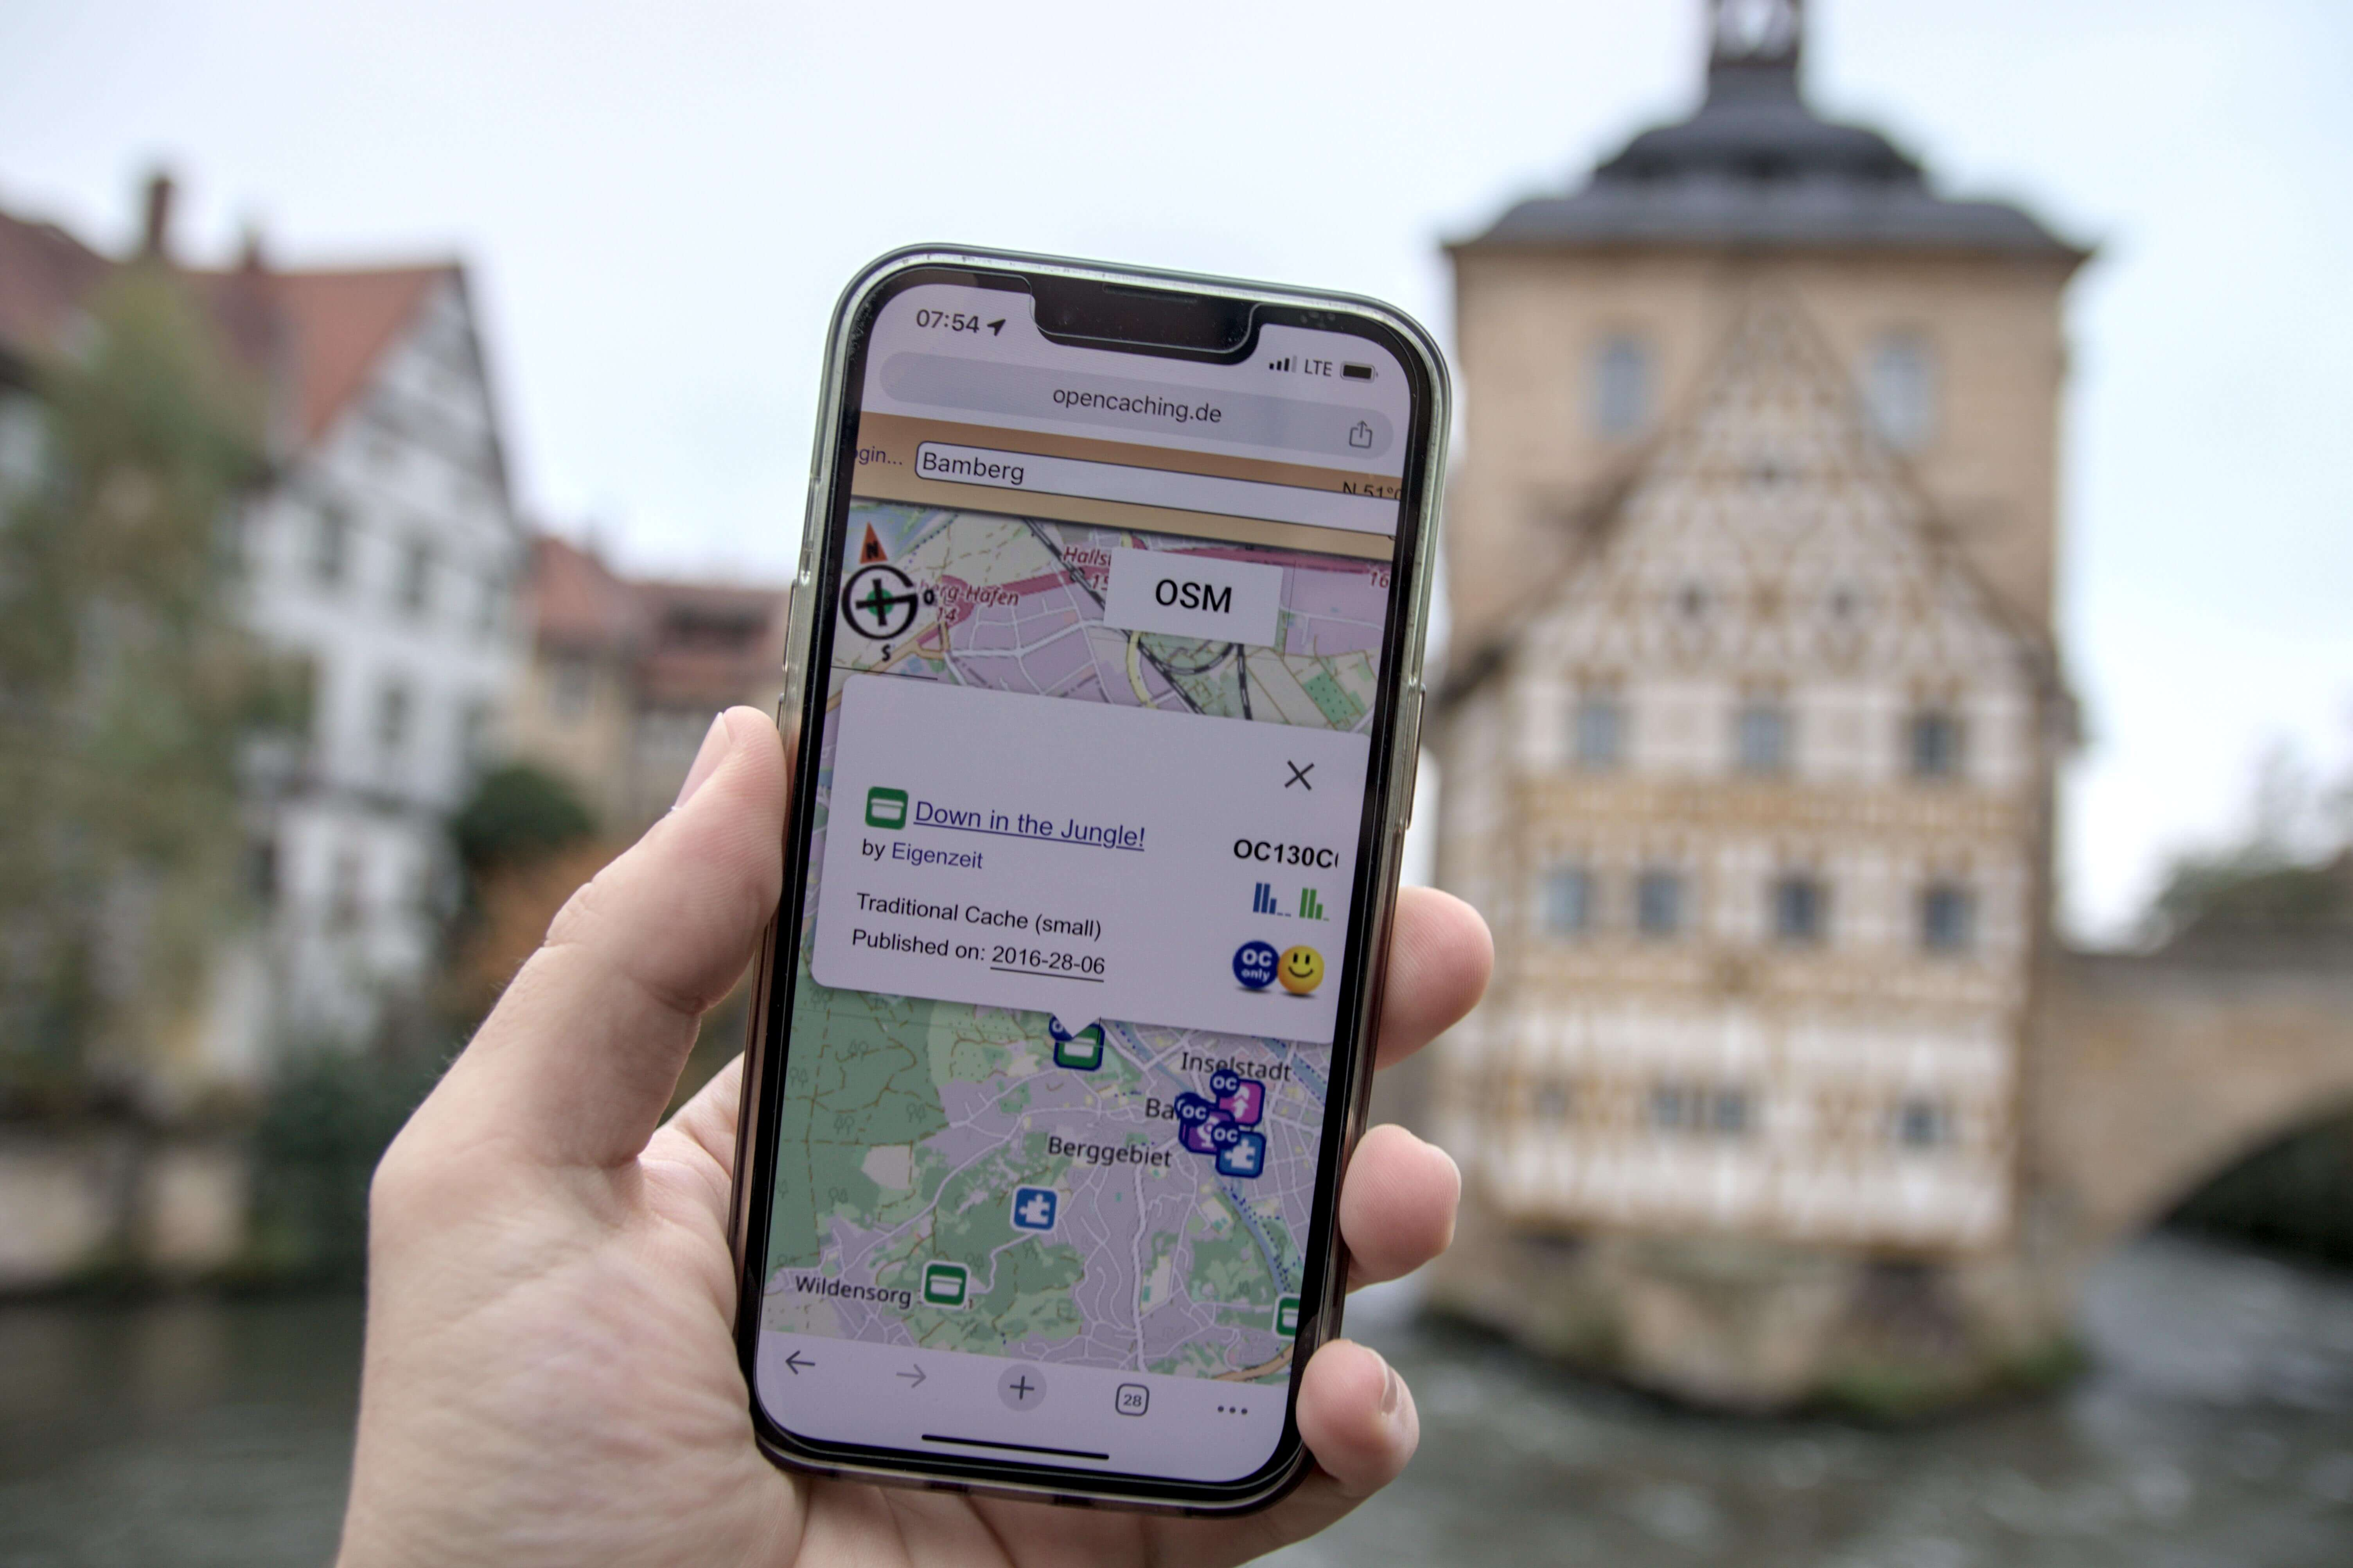
\includegraphics[width=0.7\textwidth]{figures/geocaching/first/IMG_3081.jpg}
\end{figure}

Es ist kurz vor 8:00, als ich mich vom alten Rathaus aus auf den Weg mache. Der Geocache, für den ich mich entschieden habe, heißt \enquote{Down in the Jungle!}\footnote{\url{https://www.opencaching.de/viewcache.php?wp=OC130C6}}. Er soll in der Nähe des Klosters St. Michael liegen, zwar im Stadtgebiet, aber doch auf einer Grünfläche.

\begin{figure}[h]
    \centering
    \begin{minipage}{.4\textwidth}
        \centering
        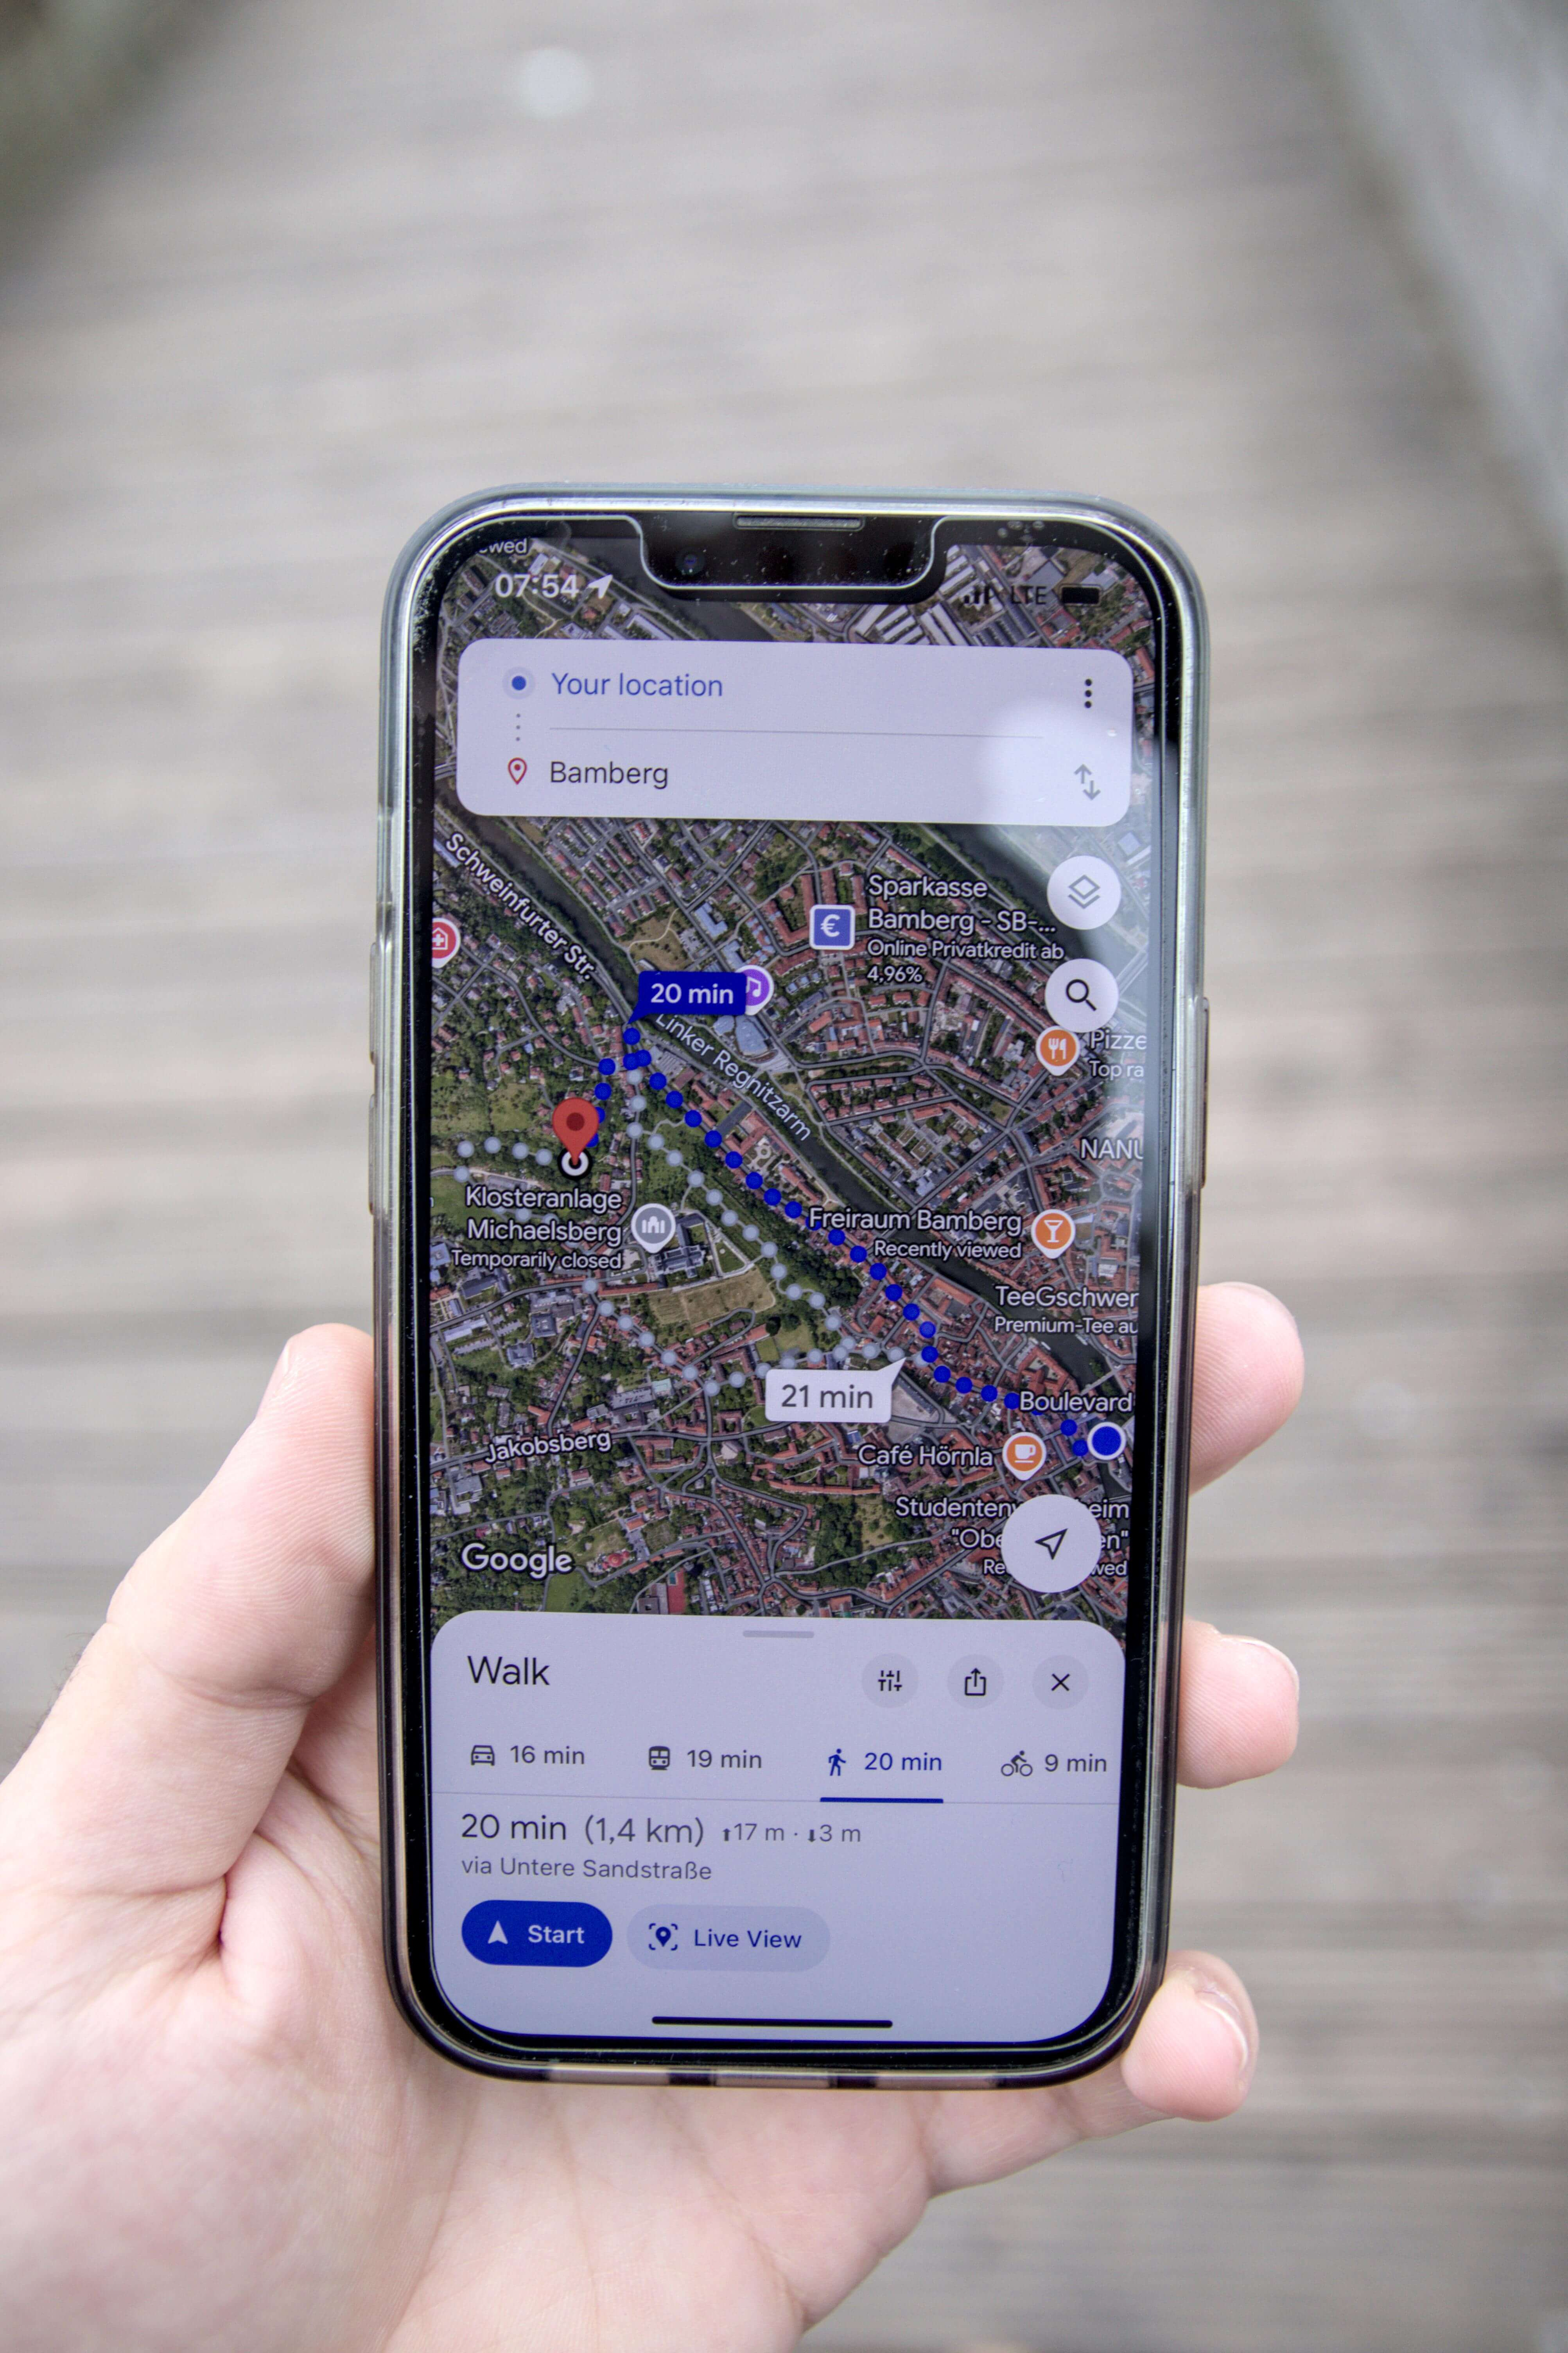
\includegraphics[width=0.7\linewidth]{figures/geocaching/first/IMG_3082.jpg}
    \end{minipage}%
    \begin{minipage}{.6\textwidth}
        \centering
        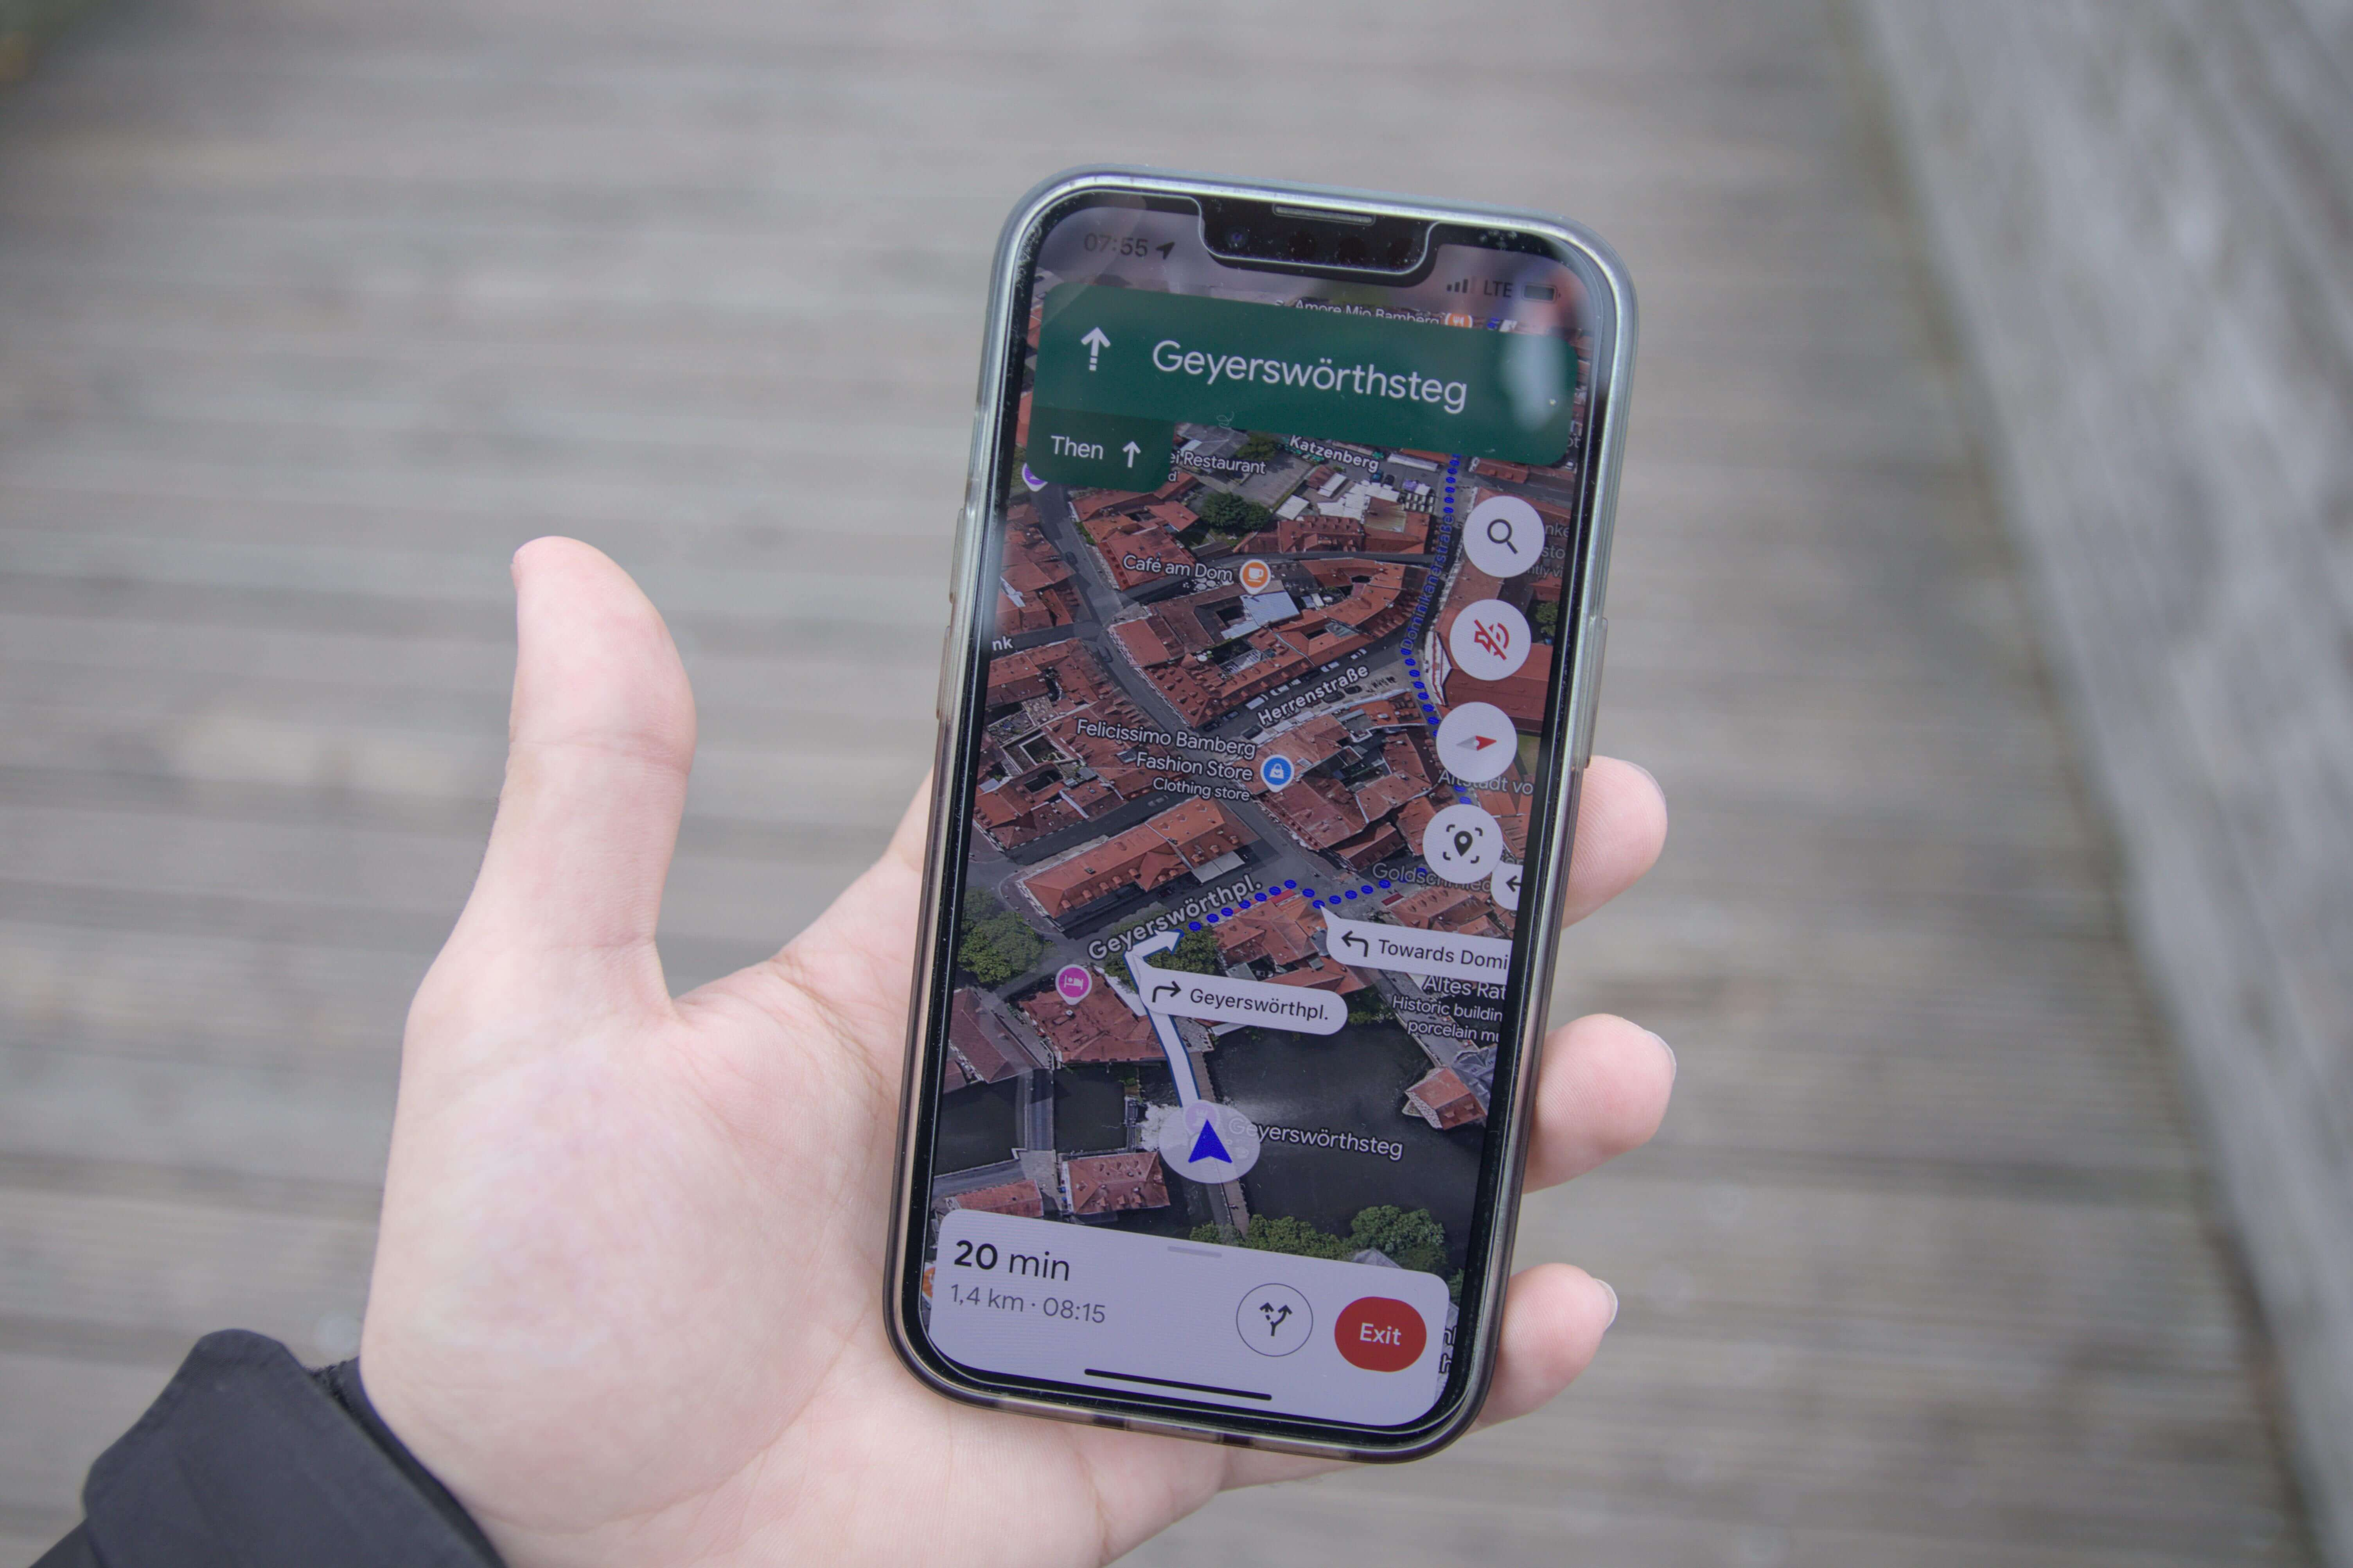
\includegraphics[width=\linewidth]{figures/geocaching/first/IMG_3085.jpg}
    \end{minipage}
\end{figure}

Ich kopiere die Koordinaten von der Internetseite, füge Sie in der mobilen App von GoogleMaps ein, starte die Navigationsfunktion und betrachte den vorgeschlagenen Weg. Ich laufe los, Richtung Sandstraße. GoogleMaps zeigt eine Routendauer von 20 Minuten an. Ab und zu werfe ich einen Blick auf mein Handy, um sicherzugehen, noch auf der korrekten Route zu sein.

Ich entscheide mich, der Alternativroute in den Grünhundsbrunnen zu folgen (siehe Abbildung \ref{first-cache-way}). An der nächsten Kreuzung werfe ich erneut einen Blick aufs Handy. Ich habe die Route noch richtig im Kopf, will aber sicher gehen. Etwa die Hälfte der Strecke ist geschafft.

In der Nähe des Klosters scheint mir eine Baustelle den Weg zu versperren. Ein Umweg ist aber nicht notwendig, für Fußgänger ist eine Querung möglich. Damit bin ich raus aus der Stadt, befinde mich in einer Parkanlage (siehe Abbildung \ref{first-cache-baustelle}). Ein Spaziergänger mit Hund kommt mir entgegen.

Noch ein Blick aufs Handy, neben der Einfahrt auf ein privates Grundstück geht ein Weg ab (siehe Abbildung \ref{first-cache-ziel}). Der Name des Caches ist treffen gewählt, man fühlt sich zwischen den Bäumen wirklich fast wie im Jungle. Nur noch Hundert Meter, laut GoogleMaps. Die Markierung auf der Karte zeigt auf einen Knick im Weg, neben einem kleinen Teich steht ein eindrucksvoller Baum. Der Zulauf zum Teich ist mit einem Geländer gesichert (siehe Abbildung \ref{first-cache-gelaende}).

Ich stecke das Handy weg, dessen Arbeit ist erst einmal getan. Jetzt heißt es: Suchen. Ich begutachte das Geländer, die Rohre beim Zulauf des Teiches, besonders den Baum. Ist hier die Dose versteckt? Möglichkeiten gäbe es auf jeden Fall, der Baum scheint am vielversprechendsten.

\begin{figure}[H]
    \centering
    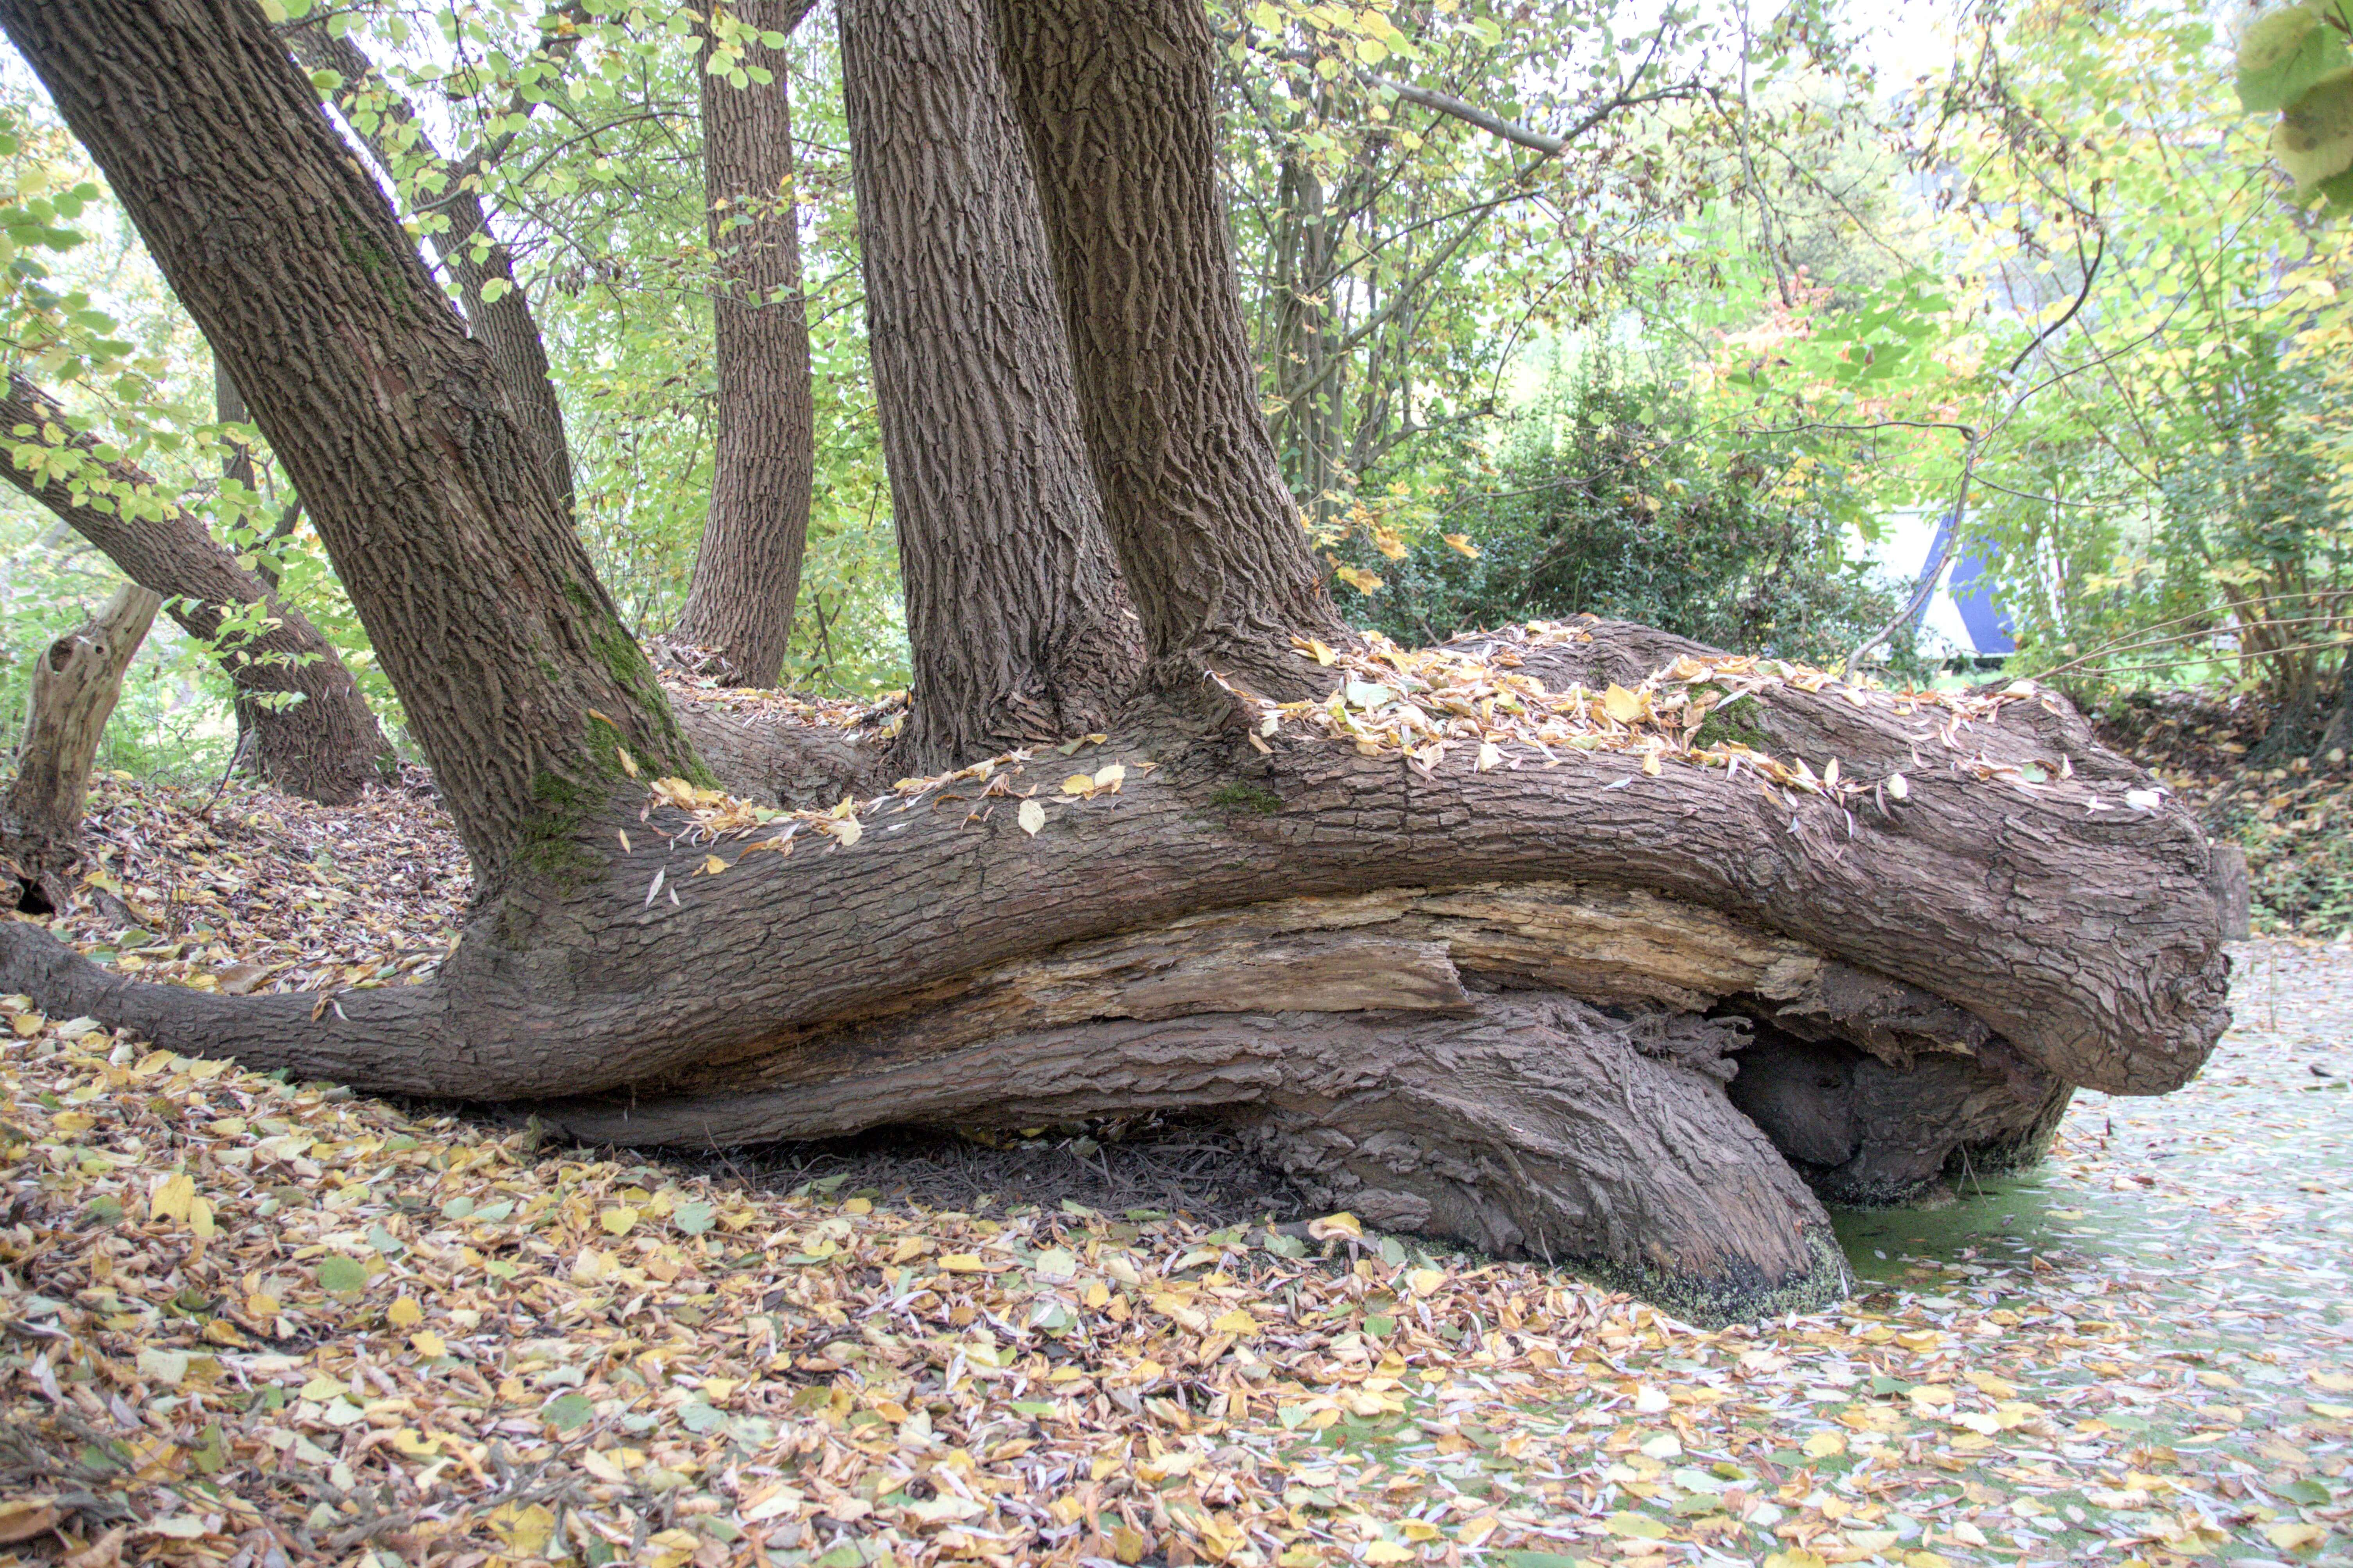
\includegraphics[width=0.7\textwidth]{figures/geocaching/first/IMG_3104.jpg}
\end{figure}

Das Herbstlaub erschwert die Suche, mit den Händen schiebe ich es zur Seite, um in Kuhlen und Astgabeln nachzusehen. Die Beschreibung des Caches bietet auch keine weiteren Anhaltspunkte. Die Kommentare geben mir kaum Anlass zur Hoffnung: Der letzte dokumentierte Fund ist bereits drei Jahre her. In der Zeit kann viel passiert sein.

Ich werfe erneut einen Blick auf die Karte: Keine Zweifel, hier muss es sein. Nach circa 25 Minuten breche ich die Suche ab, zu hoch die Wahrscheinlichkeit, dass sich die Dose nicht mehr hier befindet.

\subsection*{Schweinskopf al dente}

\begin{figure}[H]
    \centering
    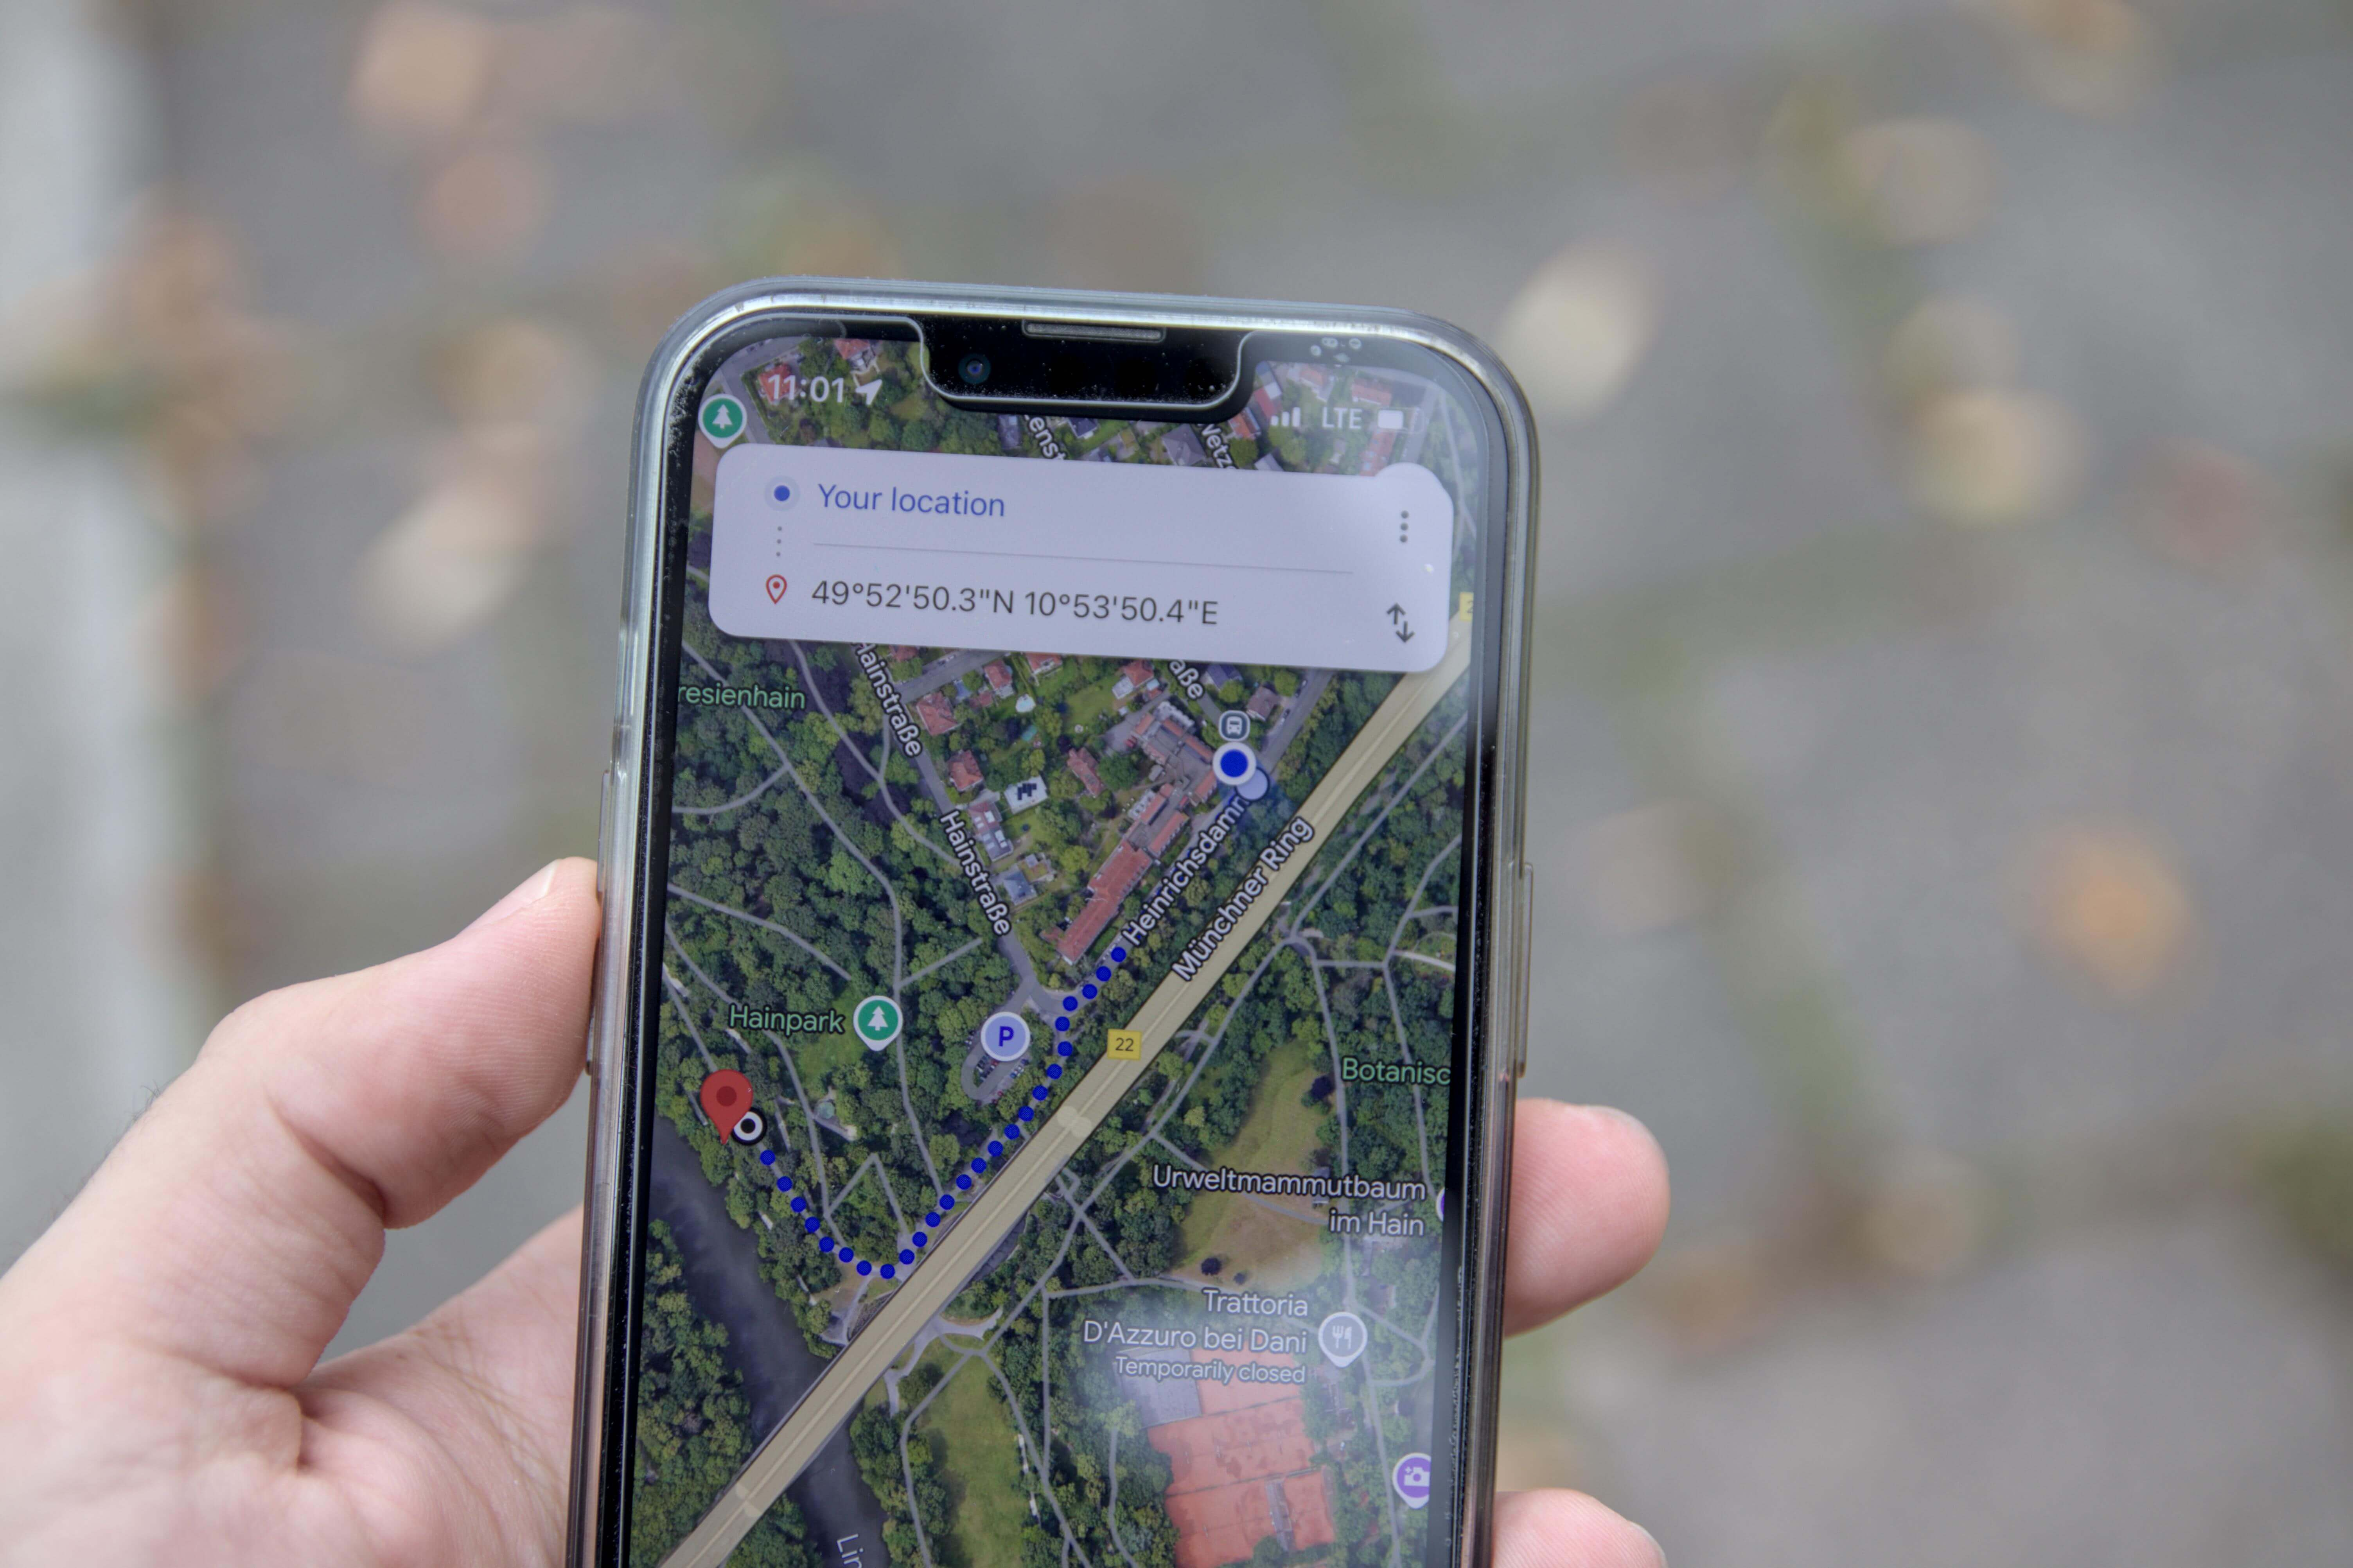
\includegraphics[width=0.7\textwidth]{figures/geocaching/second/IMG_3105.jpg}
\end{figure}


Mittags mache ich mich auf den Weg zum zweiten Versuch, diesmal aber an einem anderen Ort. Mit dem Bus geht es Richtung Hain, zum \enquote{Schweinskopf al dente}\footnote{\url{https://www.opencaching.de/viewcache.php?wp=OC141A5}}. Der letzte Eintrag ist hier vom 26. März 2024, die Chancen sollten also ganz gut stehen, dass dieser Cache noch zu finden ist.

Von der Haltestelle Wilhelm-Löhe-Heim aus geht es zu Fuß weiter. Das Prozedere ist dasselbe wie beim ersten Versuch: Koordinaten in GoogleMaps einfügen, Zielführung starten und los geht's.

Erneut entscheide ich mich für eine alternative Route. Der exakte Ort scheint auf der Karte näher an dem direkt am Wasser verlaufenden Weg zu liegen, als an dem Weg, auf den mich die Navigation führen will. Diesem Weg folge ich also noch etwas, dann bin ich angekommen (siehe Abbildung \ref{second-cache-weg}).

Die Koordinaten liegen rechts des Weges, was auch Sinn macht: Links folgt auf die Böschung direkt die Regnitz, hier gibt es kaum Möglichkeiten, eine Box zu verstecken. Rechts hingegen Bäume, Sträucher, Wurzeln.

\begin{figure}[H]
    \centering
    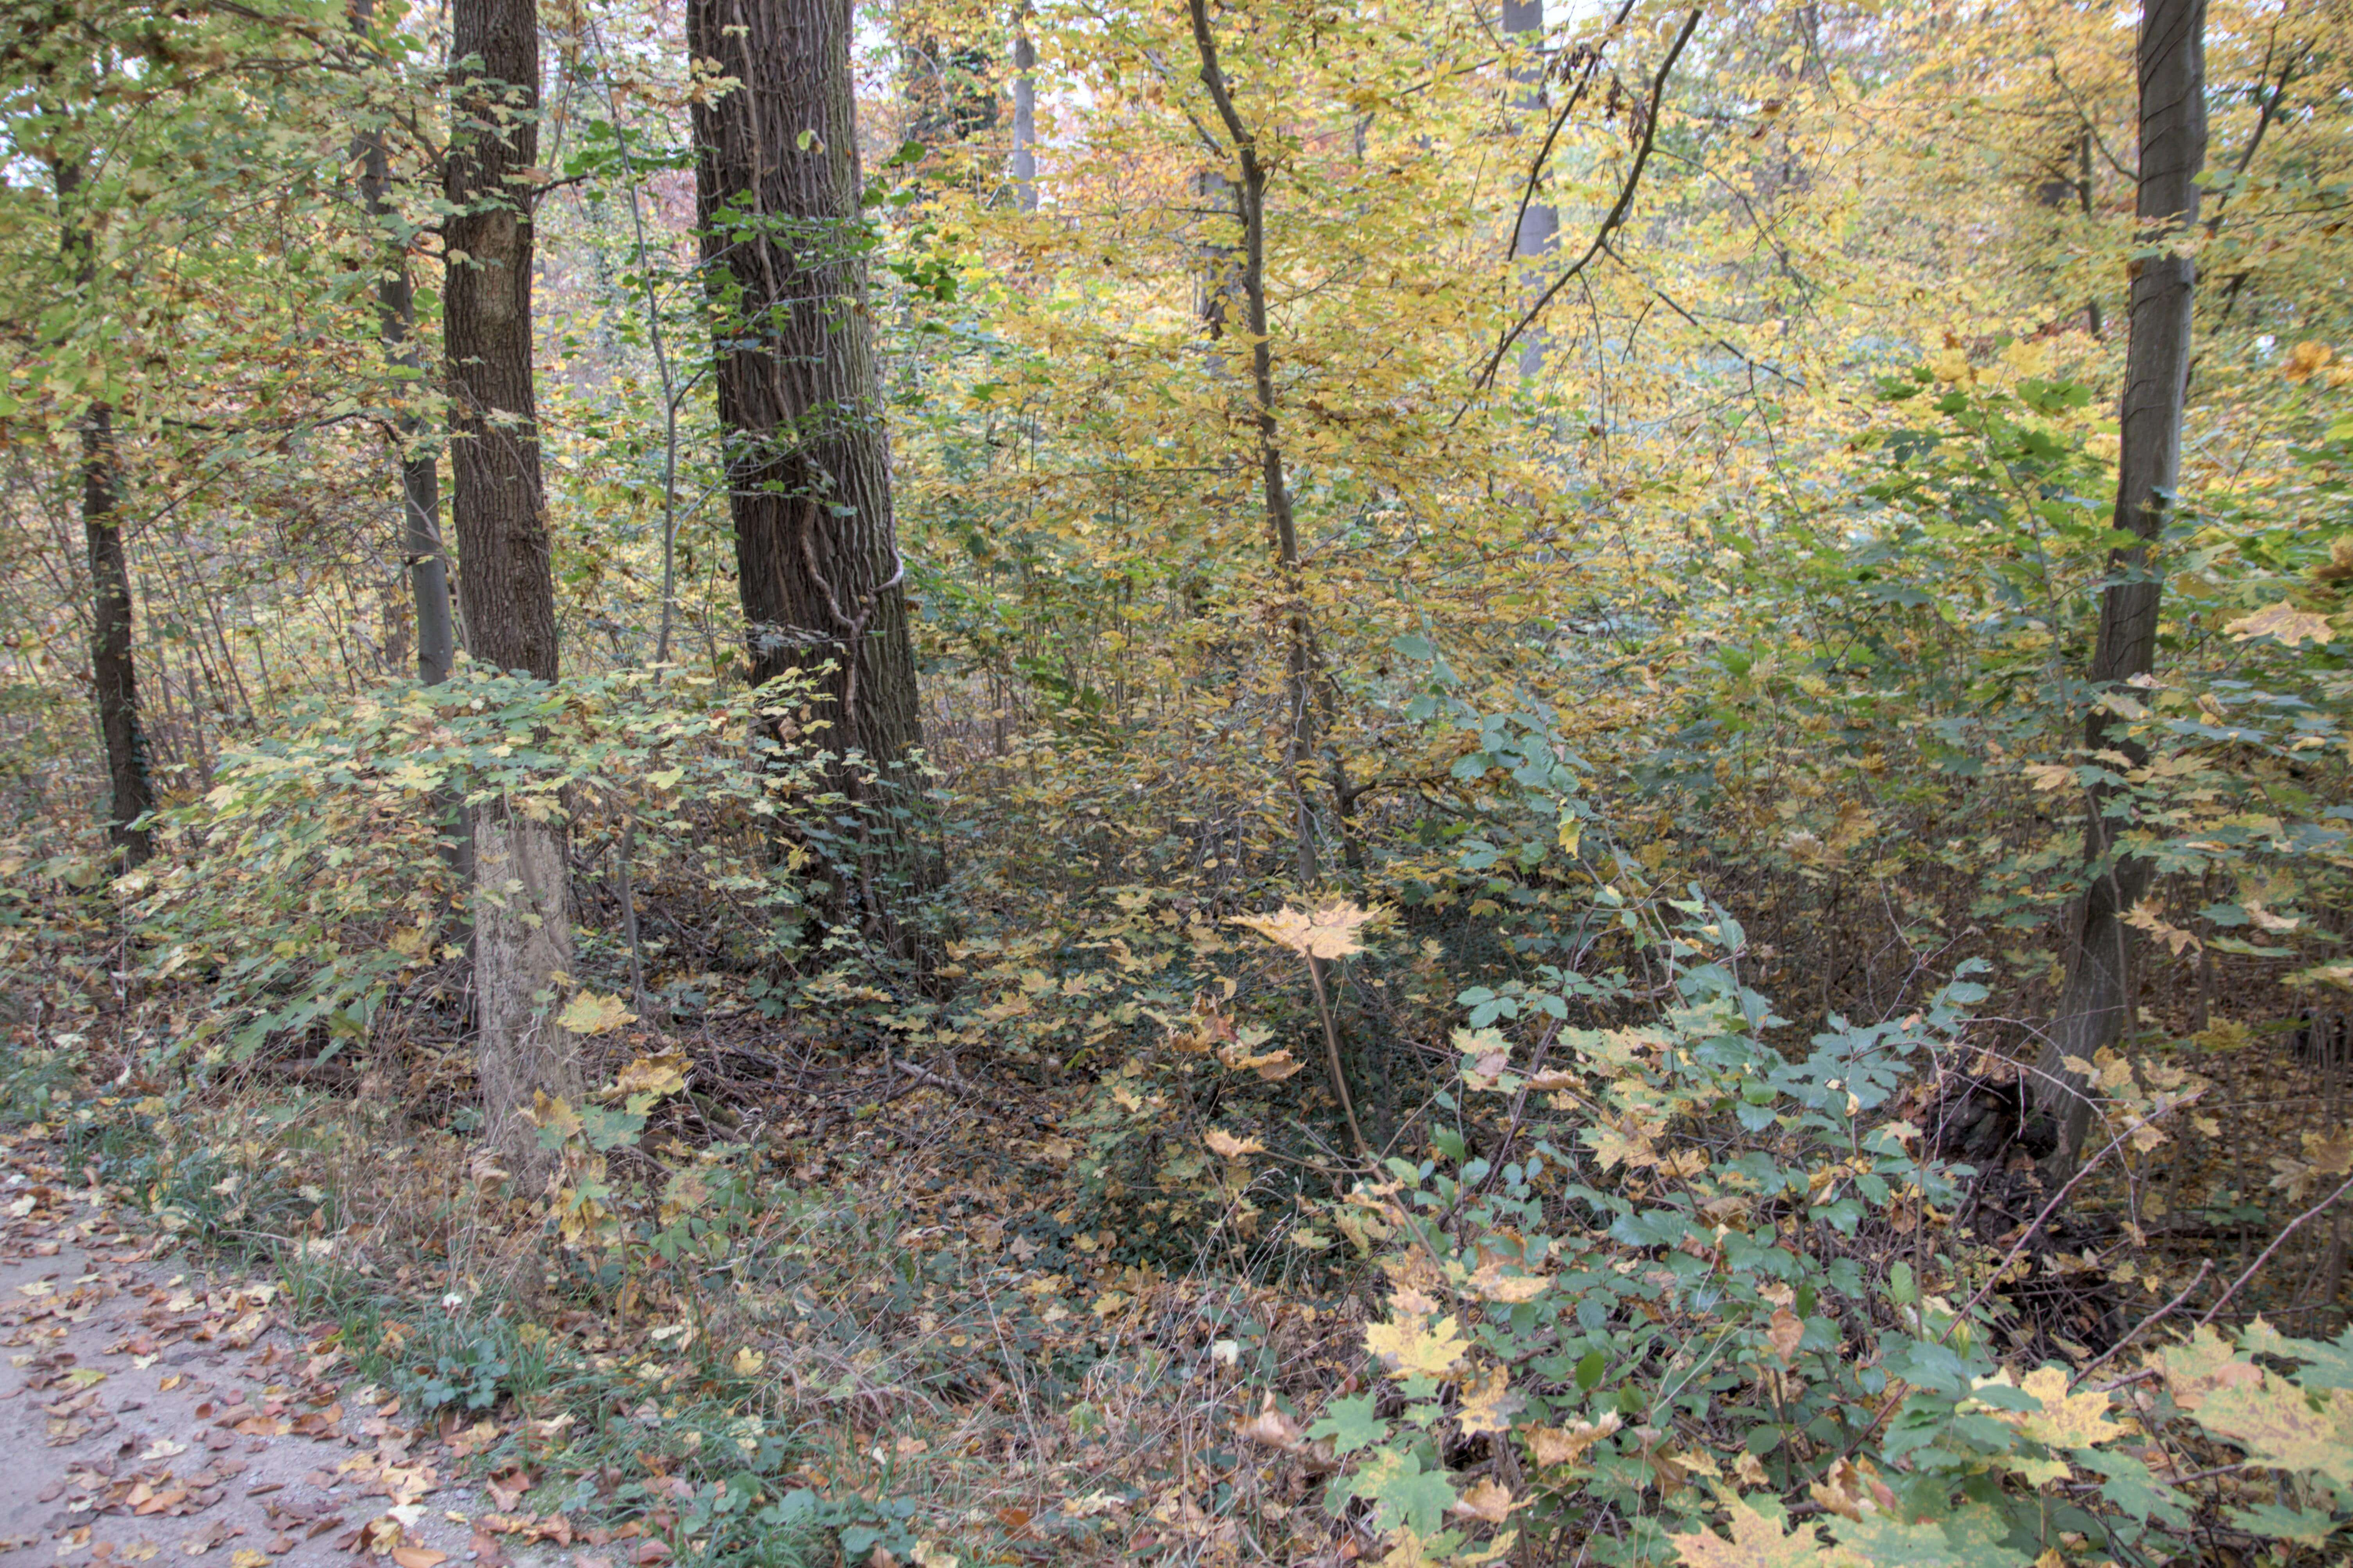
\includegraphics[width=0.5\textwidth]{figures/geocaching/second/IMG_3114.jpg}
\end{figure}


Also stecke ich wieder mein Handy weg und mache mich auf die Suche. Wieder fällt mein Blick zuerst auf einen kräftigen Baum, ich suche die Wurzeln ab, suche nach Höhlen oder Astgabelungen. Als ich hier nicht fündig werde, streift mein Blick durch die Umgebung. Glücklicherweise sind kaum andere Personen unterwegs, auf die ich Rücksicht nehmen müsste.

Mein Blick bleibt an einem Baumstumpf hängen. Da sollte es doch auch ein paar gute Verstecke geben. Ich umrunden das Objekt, streiche erneut Laub beiseite. Und tatsächlich, bei der zweiten Umrundung werde ich fündig (siehe Abbildung \ref{second-cache-versteck}). Am Anfang muss ich den grünen Deckel der Box noch übersehen haben, der nun zwischen Rinde und Laub hervorlugt.

\begin{figure}[H]
    \centering
    \begin{minipage}{.5\textwidth}
        \centering
        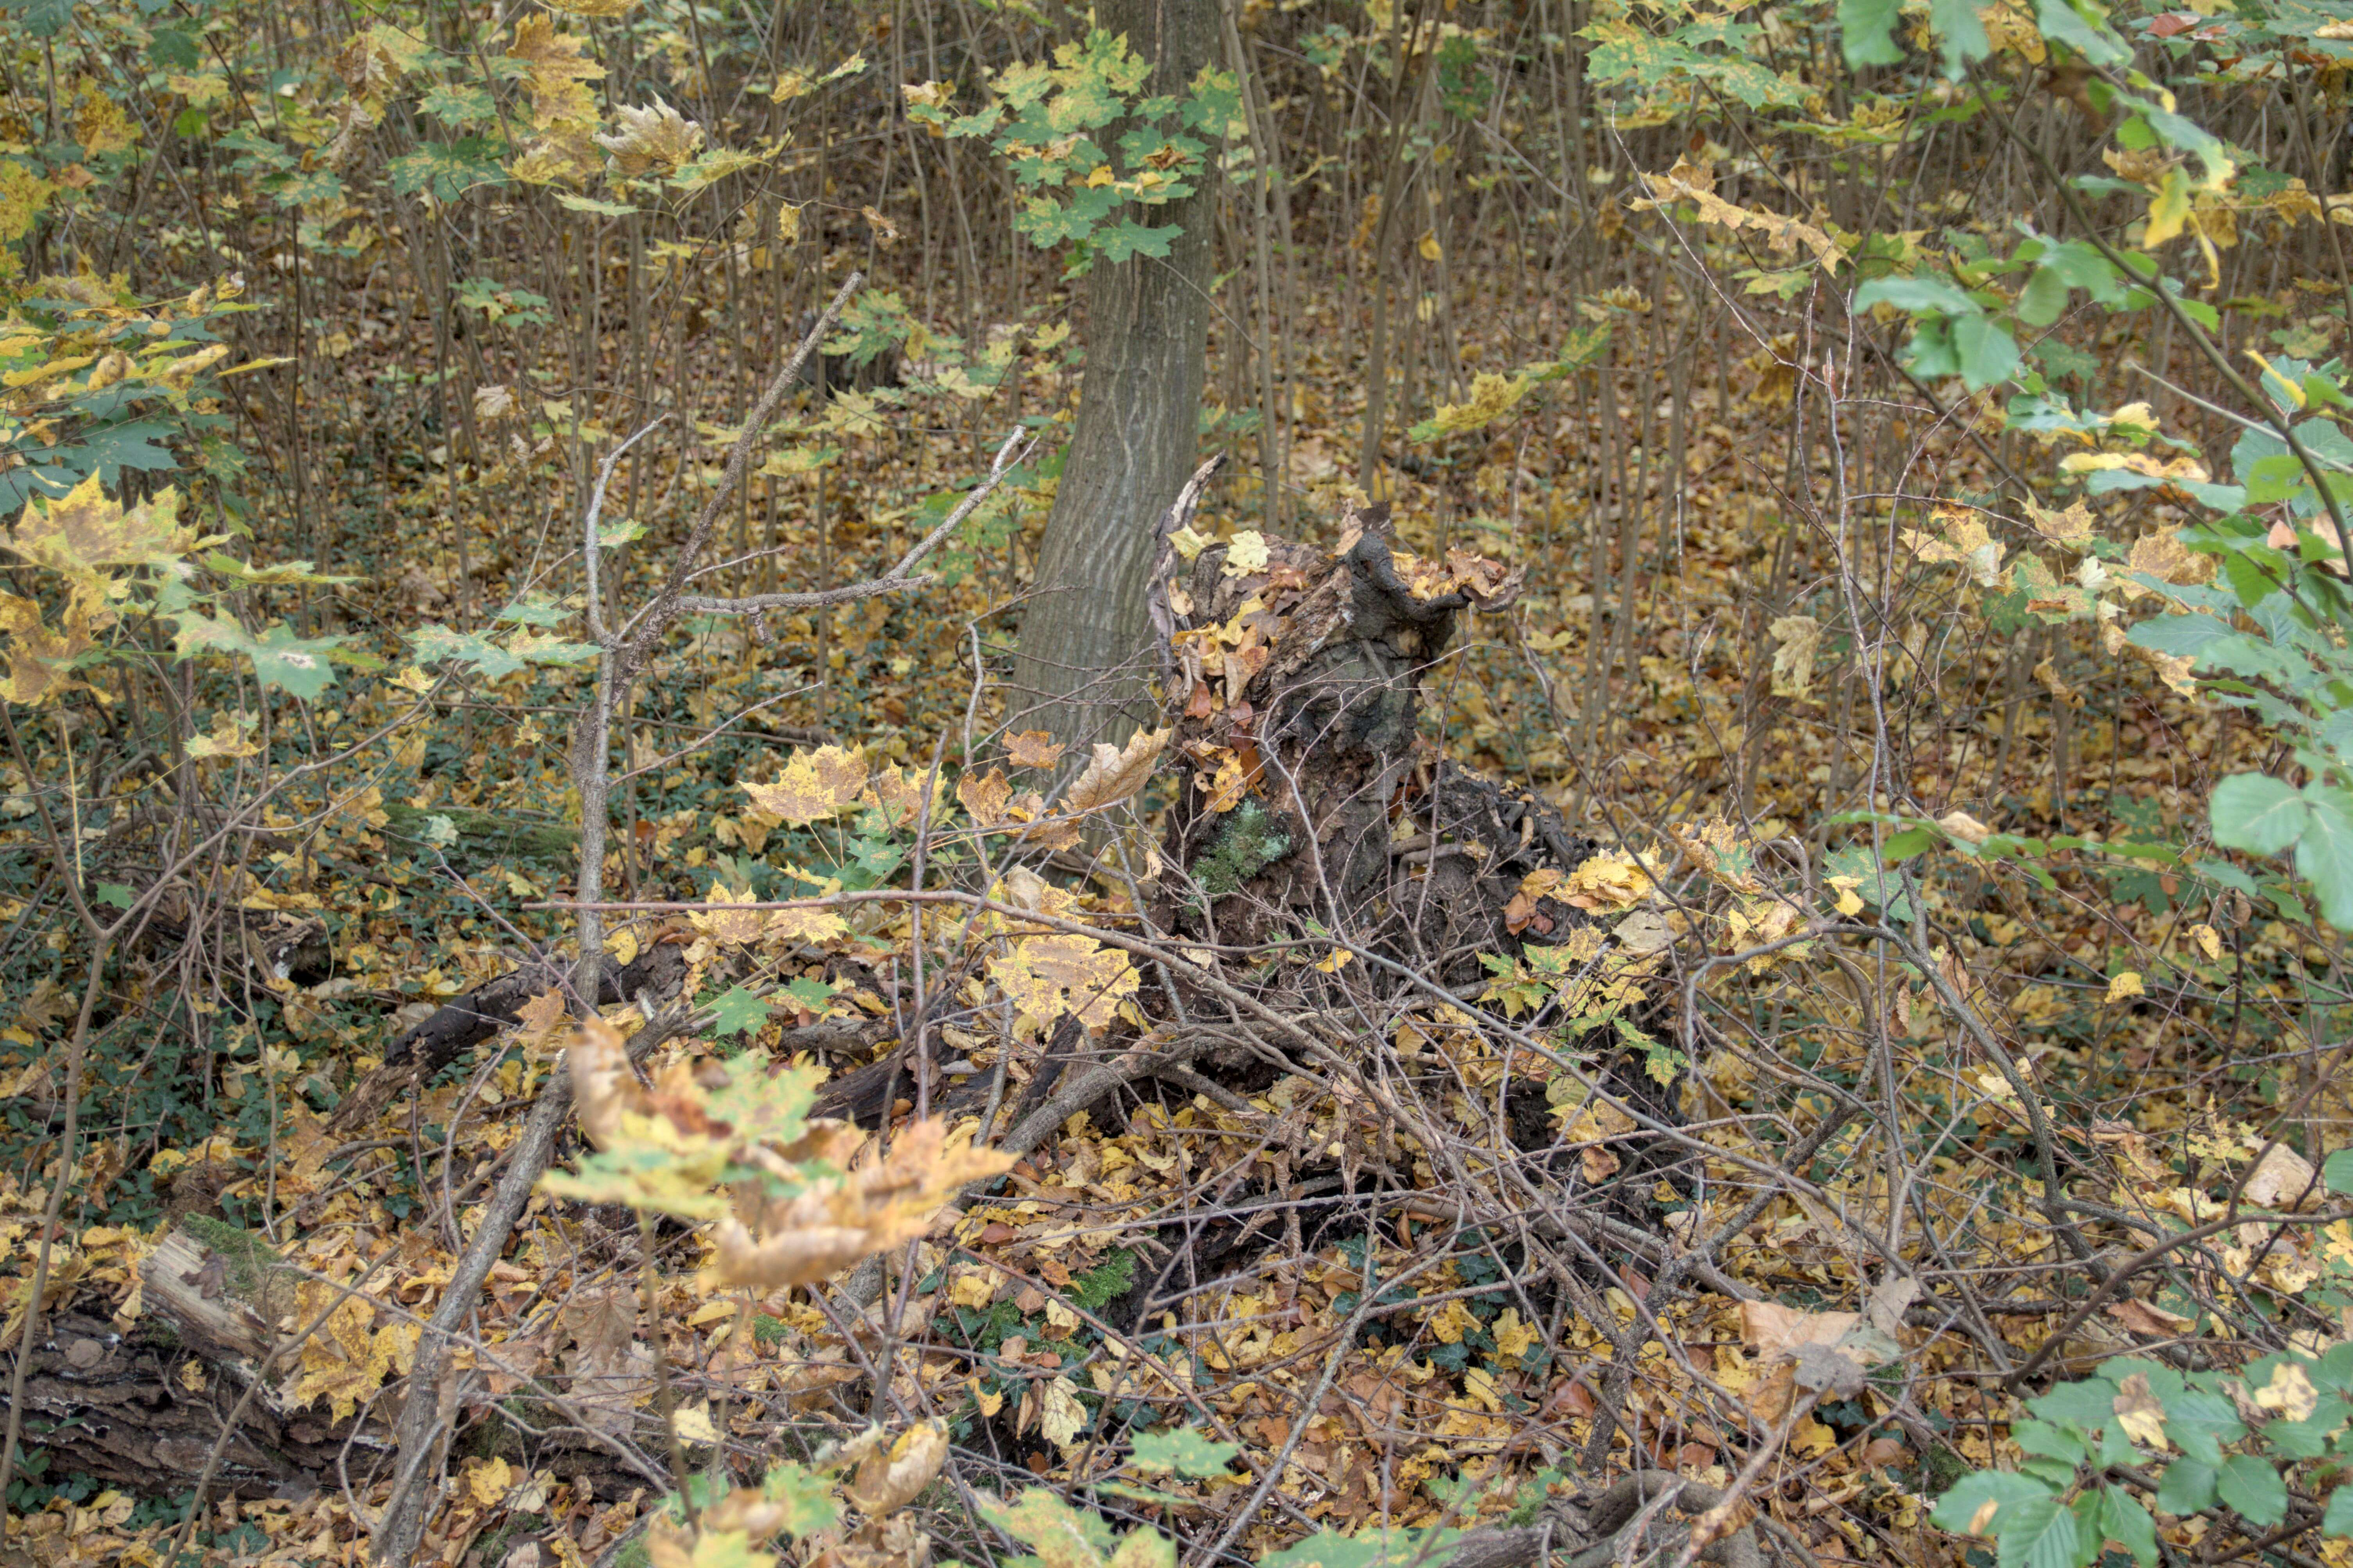
\includegraphics[width=.95\linewidth]{figures/geocaching/second/IMG_3116.jpg}
    \end{minipage}%
    \begin{minipage}{.5\textwidth}
        \centering
        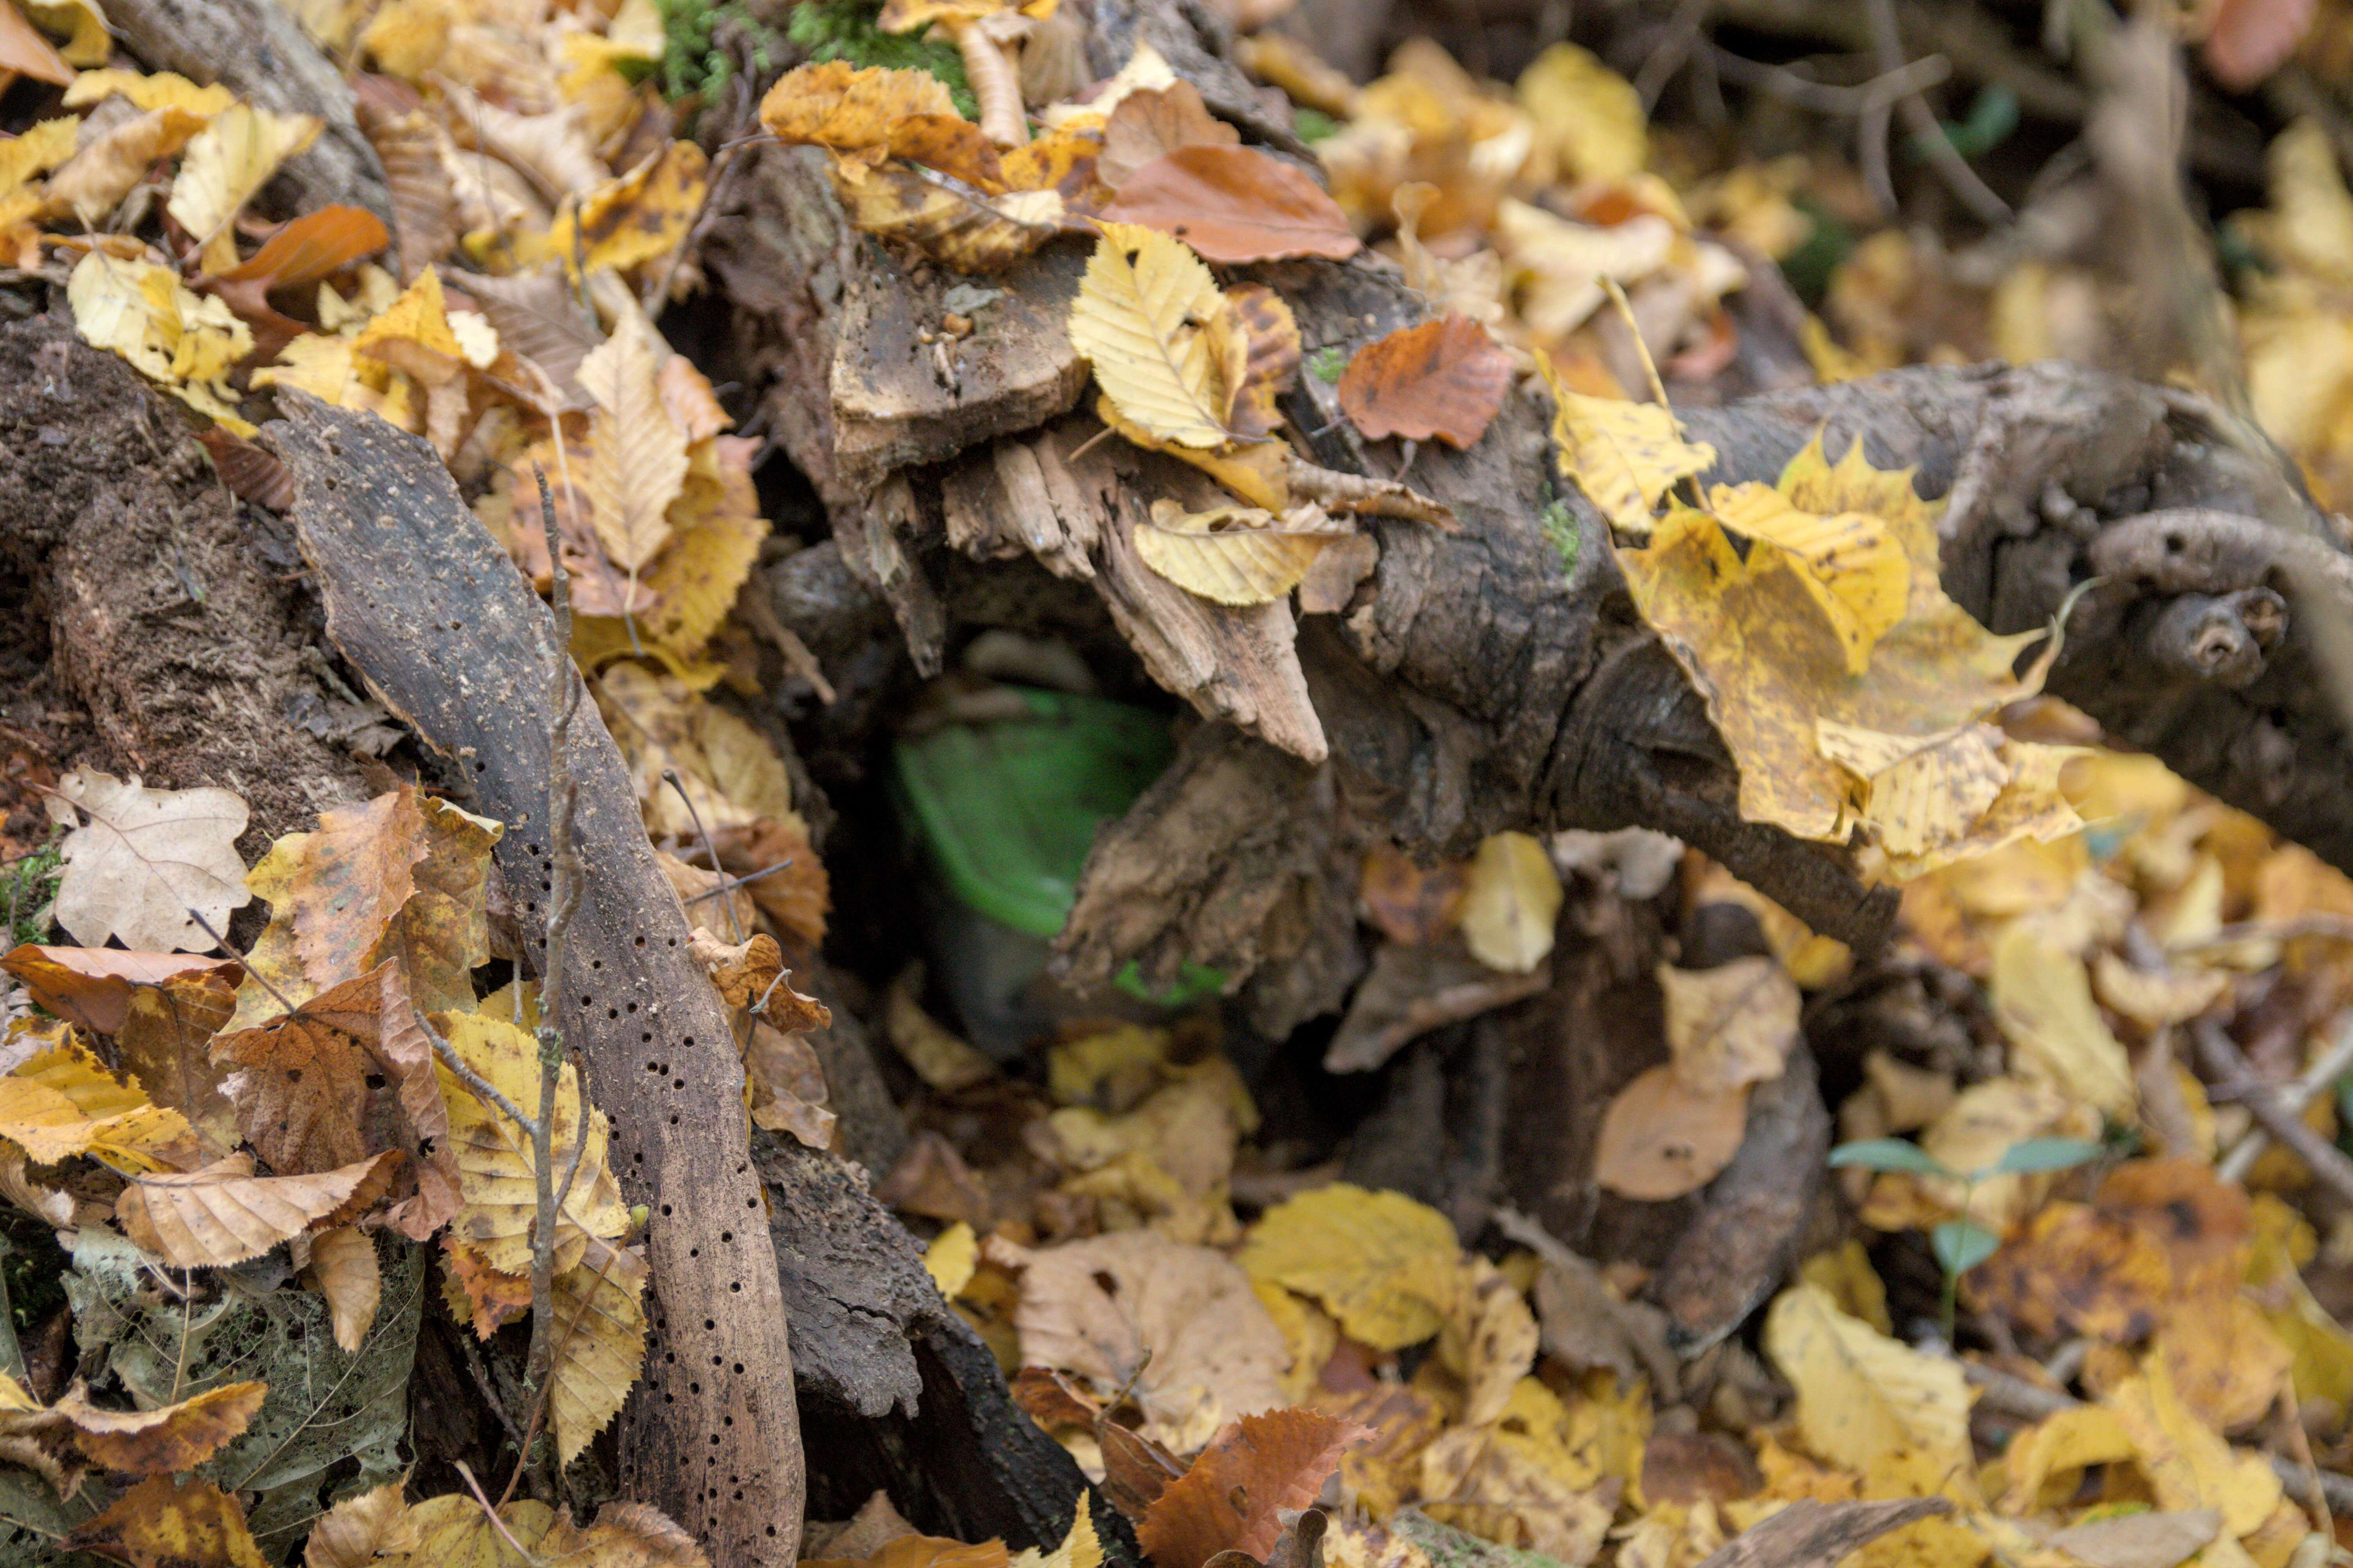
\includegraphics[width=.95\linewidth]{figures/geocaching/second/IMG_3110.jpg}
    \end{minipage}
    \caption{Der Baumstumpf, an dessen Rückseite die Box versteckt ist.}

\end{figure}

Ich nehme die Box aus ihrem Versteck und öffne sie. Ich blättere durch das etwas feuchte, leicht gammelige Logbuch und trage das Datum und meinen Namen ein (Abbildung \ref{second-cache-log}). Anschließend lege ich es zurück und platziere die Box an dem Ort, an dem ich sie wenige Minuten vorher gefunden habe.

\subsection*{Zusammenfassung}
Die Interaktion mit dem Smartphone findet überwiegend auf dem Weg zum groben Suchort statt. Vor Ort habe ich das Handy kaum benutzt, da die Genauigkeit der Koordinaten und des GPS Signals nicht ausreicht, um den Cache exakt zu lokalisieren, hier ist dann doch die Suche per Hand gefragt. Ein oder zweimal habe ich während der Suche dann doch einen Blick aufs Handy geworfen, um die Position der Koordinaten mit meinem standort abzugleichen oder einen Blick auf die Beschreibung des Geocaches zu werfen. Dadurch wird die Suche auch zu einer interessanten Kombination aus Technik und Natur, der technisch unterstützten Wegsuche und dem händischen Suchen, im Herbst schon fast Wühlen, vor Ort.

Problematisch war vor allem das Herbstlaub, das die Suche erschwerte. Die Beschreibungen der Caches waren nicht wirklich hilfreich, da sie, wenn überhaupt, nur grobe Hinweise auf den Versteckort geben.

Beide Caches haben einen starken Bezug zu ihrer Umgebung. Beim ersten war das bereits durch den Titel deutlich, der ja wirklich gut auf die Ort gepasst hat.Auch wenn ich die Dose nicht finden konnte: Falls sie noch vor Ort ist, muss sie in einer starken Beziehung zur Umgebung stehen, beispielsweise eine Höhle in dem auffälligen Baum ausnutzen. Auch der zweite Cache war in der Nähe von Bäumen versteckt, was auch sinnvoll ist: Einerseits gibt es hier einfach besonders viele Versteckmöglichkeiten, andererseits ist die Chance gering, dass der Cache von anderen Personen gefunden wird, die nicht gezielt danach suchen.